\documentclass[paper=A4,pagesize=auto,12pt,headinclude=true,footinclude=true,BCOR=0mm,DIV=calc]{scrartcl}
\usepackage[english]{babel}
\usepackage[utf8]{inputenc}
\usepackage{graphicx}
\usepackage{geometry}
\usepackage[T1]{fontenc}
\usepackage{lmodern}
\usepackage{amsmath}
\usepackage[scaled]{uarial}
\usepackage{blindtext}
\usepackage{hyperref}
\usepackage{eurosym}
\usepackage{color}
\usepackage{subfigure}
\usepackage{listings}
\usepackage{float}
\usepackage{amsfonts}
\usepackage{amssymb}
\usepackage{graphics}
\usepackage{wrapfig}
\usepackage{setspace}
\usepackage[font=footnotesize]{caption}
\usepackage[format=plain,
justification=RaggedRight,
singlelinecheck=false]
{caption}
\usepackage{textcomp}
\geometry{
	left=2.5cm,
	right=2.5cm,
	top=2.5cm,
	bottom=2cm,
}
\makeatletter
\newcommand{\MSonehalfspacing}{%
	\setstretch{1.44}%  default
	\ifcase \@ptsize \relax % 10pt
	\setstretch {1.44}%
	\or % 11pt
	\setstretch {1.44}%
	\or % 12pt
	\setstretch {1.44}%
	\fi
}
\MSonehalfspacing
\setlength{\parindent}{0pt}

\begin{document}
	
	\title{Github Repository Classifier}
	\author{\textbf{Rami Aly$^{1}$, Andre Schurat}$^{2}$\\
		$^{1}$ University of Hamburg\\
		$^{2}$ Technical University of Dortmund}
	\maketitle
	
	\newpage
	
	\section{Abstract}
	
	
	\newpage
	
	\tableofcontents 
	
	\newpage
	\section{Selecting features} 
	\subsection{General thoughts}
	At the early beginning of our process we discussed about our selection of Features. It was clear to us that it is not possible to manually enclose the available data sets in a way where we wouldn’t miss important features. So we decided to not cut down the data sets, instead we condoned gathering statistically irrelevant informations so far. In the further context we will call this phenomena “information noise”.
	\subsection{Selected features}
	For a better visualization of  created a graphic:
	\\
	INSERTPICTURE
	\\
	The entries with a double circle represent our features. In the further process we explain our decision to choose this ones and why we didn’t choose other.
	Why we choose these features and didn’t choose other ones will be explained in detail in the further process.
	
	The next section is used to explain our decision behind our feature selection, and why we didn’t use other ones, although we considered them. 
	
	\subsubsection{Word Count}
	The word count represents our most important feature. It is defined as the occurrence of each word contained in any text across the whole repository. This includes all readable text files, and text contained in PDF, Word and Powerpoint files. The contents of the readme file count 10 times as much since it contains the most important information the most cases. 
	We choose this feature because the Word Count represents the repository’s content in really wide way. At this point we keep in mind that at the backside the information noise especially for the word count is immense. 
	An example of a Word Count Table can be found inside the attachments. TODO
	
	
	\subsubsection{File Ending Count}
	
	The File Ending Count is defined as the occurrence of different file endings in the whole repository. We choose this feature because file endings reflect the use of different programming languages and other file formats in the best possible way.
	
	\subsubsection{Filename Count}
	
	Just like the File Ending Count the Filename Count is defined as the occurrence of different file and folder names in the whole repository.
	We choose this feature because there are several key files and folders which militate in favor of a specific category.        
	
	\subsubsection{Media Density}
	
	The Media Density describes ratio from the total count of media files to the total word count contained inside the Word Count. Media files contained inside PDF, Word. Zip and Powerpoint files are counted as well. We choose this feature because there are specific repository categories that tend to use more or less media files.
	
	\subsubsection{The Github Rate Limit}
	The data available by a simple web browser is huge but since not of all it may accessible via code we took a look into the Github API instead. This offered a major problem: The Github API only allows 60 unauthenticated requests per hour and 5000 for authenticated ones(1). Even if we take in count that only authenticated requests are used, which would require each user to own a github account, 5000 requests per hour are not enough to analyze hundreds of Repositories per hour. There Repositories with over 500.000 commits and a single github request returns only the first 500. So we would need 1000 request for a single repository just to get all of the commits. So our conclusion so far is that we need to collect our features with as little requests as possible.
	
	
	
	\section{Gathering selected features from Github}
	
	
	
	\section{Removing irrelevant information from selected features}
	Especially the features \textit{File Ending Count}, \textit{Word Count} and\textit{ Filename Count} still consists of information noise as every repository could contain words that are unique to every other repository and as such not relevant for the classification. Then again some words could be in almost every repository but their occurrence does not differentiate between the classes in a considerable margin. Due to the rising complexity of a neural network for every input added to it one should desire to find a balance between the number of words and the relevance of a word for classification. We decided to create a dictionary for each of the mentioned three features that contains every relevant word for classification. 
	
	Of course the question arises on how to chose the words for the dictionaries. For this we created an algorithm.
	
	The algorithm takes classified repositories, we choose to use our \hyperref[sec:Training Set]{Training Datasets}.
	In the first step the intersection with a threshold $p$ of words between repositories of the same class is calculated for each repository class. The threshhold $p$ is used to define the minimum ratio between repositories that contain the word and the total number of repositories in the class. 
	This step is used to filter words that are too unique.
	
	
	\section{Building the Prediction Model}
	
	\subsection{Choosing a prediction Model}
	Of course there are many different approaches to the problem. A static algorithm to classify repositories is rather impractical because the parameters of our classify function would be strongly influenced by our interpretation of weights of the features for each class. However we quickly noticed that the complexity is very high, so that a normal algorithm would limit the aspects which possibly needed be considered. The problem is non-linear and through the static analysis we would loose the possibility to freely improve or change the classifier. As the software and use-case market of Github rises the possible need of further classes could arise.
	
	Hence to ensure a classifier who is as dynamic and as extensible as possible we choose to use some form of machine learning.
	The problem which needs to be solved by the Prediction Model is a classification problem: We have a fixed number of values for selected features as input and as an output the class to which the values fit the most. As a result of this fact it was pretty clear to us that a supervised learning method would be optimal.
	
	In the next step we thought about the pro- and contra arguments of non-parametic and parametic learning.
	For example Gaussian-Process-Models could be used in principle, as one does not need to specify a fixed number of parameters and therefore be non-parametic. 
	The main problem with Gaussian-Process-Models is that they scale rather poorly with a complexity of $O(n^{3})$ \cite{DukeUniversity}. Moreover if we keep the huge dimension of repository datasets in mind and as such the possible complexity of the classifier function, our choice will lead us to a parametric neural Network. A neural network combines every important aspect from above and is furthermore capable of performing good in presence of imprecise and especially of noisy data.
	
	\subsection{Our Neural Network Model}
First of all for our selected features it is not needed to consider temporal behavior. We do need need to save an internal state (If we had used a sequence of commits this could have been otherwise). It should be fully sufficient to use a Feed-forward neural network.

As for a Neural Network with supervised learning we choose that a Multilayer perceptron(MLP) with one hidden Layer would be sufficient for our classification problem. We already mentioned that our classification problem is not linear. Hence at least one hidden Layer is required to solve the problem. Furthermore we know that this MLP can approximate any bounded continuous function with arbitrary precision \cite{ApproximateAnyFunction}, particularly our classification problem.
The usage of a linear activation function would result in a MLP with a set of possible functions to be equivalent those of a normal input-output perceptron. Therefore we need to use a nonlinear activation function. We therefore decided to use a Sigmoid function. 

For the training we used as expected for a MLP Backpropagation. To reduce the chance to be stuck in a local minimum we used intertia so that the previous change will influence the weight adjustment in the current round.

The neuron count for the output-layer is set to the number of different classes into which we want to classify the input. So for our Neural Network we used 7 output neurons.

Our input neurons count equals to sum of the length of every dictionary plus all relevant ratios of our selected features.

\subsection{Formating and further preprocessing of Features to fit into the Neural Network}
We tried to find the perfect balance in preprocessing so that on the one hand the network does not need to learn obvious relations between features and on the other hand not to loose possible relations by too much preprocessing.

To format the input for the neuron we will iterate through every word in a dictionary of a type. The ratio between the relative occurence of the word for this type and the occurence value stored in the dictionary is calculated. Effectively this ratio is equal to the deviation of the relative word occurrence for the considered type. In case the relative occurrence of a word ending is higher then the occurrence in the dictionary it will result into a value $> 1$. So there is still the necessity of a normalization process - for the dictionary deviation as well as for the ratios.

There are several possibilities to normalize the input. In our case it is important that the input is distinct. Furthermore standard normalize procedures are using a maximum and minimum value. The problem is that it is not possible to define an upper bound for the inputs because a testinput could always exceed the previous bound and therefore the attribute of distinction is contradicted (New Max value could lead to values to have the exact same value as a value with an old bound).
Therefore we decided to use a logistic function to normalize our data. A logistic function is monotonically increasing and thus is every value distinct. Depending wether we use a Sigmoid or tanh function we will construct the logistic function in a way that the upper bound is 1 and the lower bound respectively 0 or -1 in case of the tanh. 
We can then use a constant of proportionality to optimize the distribution of the values:

$f(x) = 2 * \frac{1}{1 + e^{-k(x-k)}} -1$

To support the understanding of our normalization technique we will plot our function for $k \in \{0.03, 1, 5\}$.\\
\begin{figure}[H]
	\subfigure{\label{konfiguration}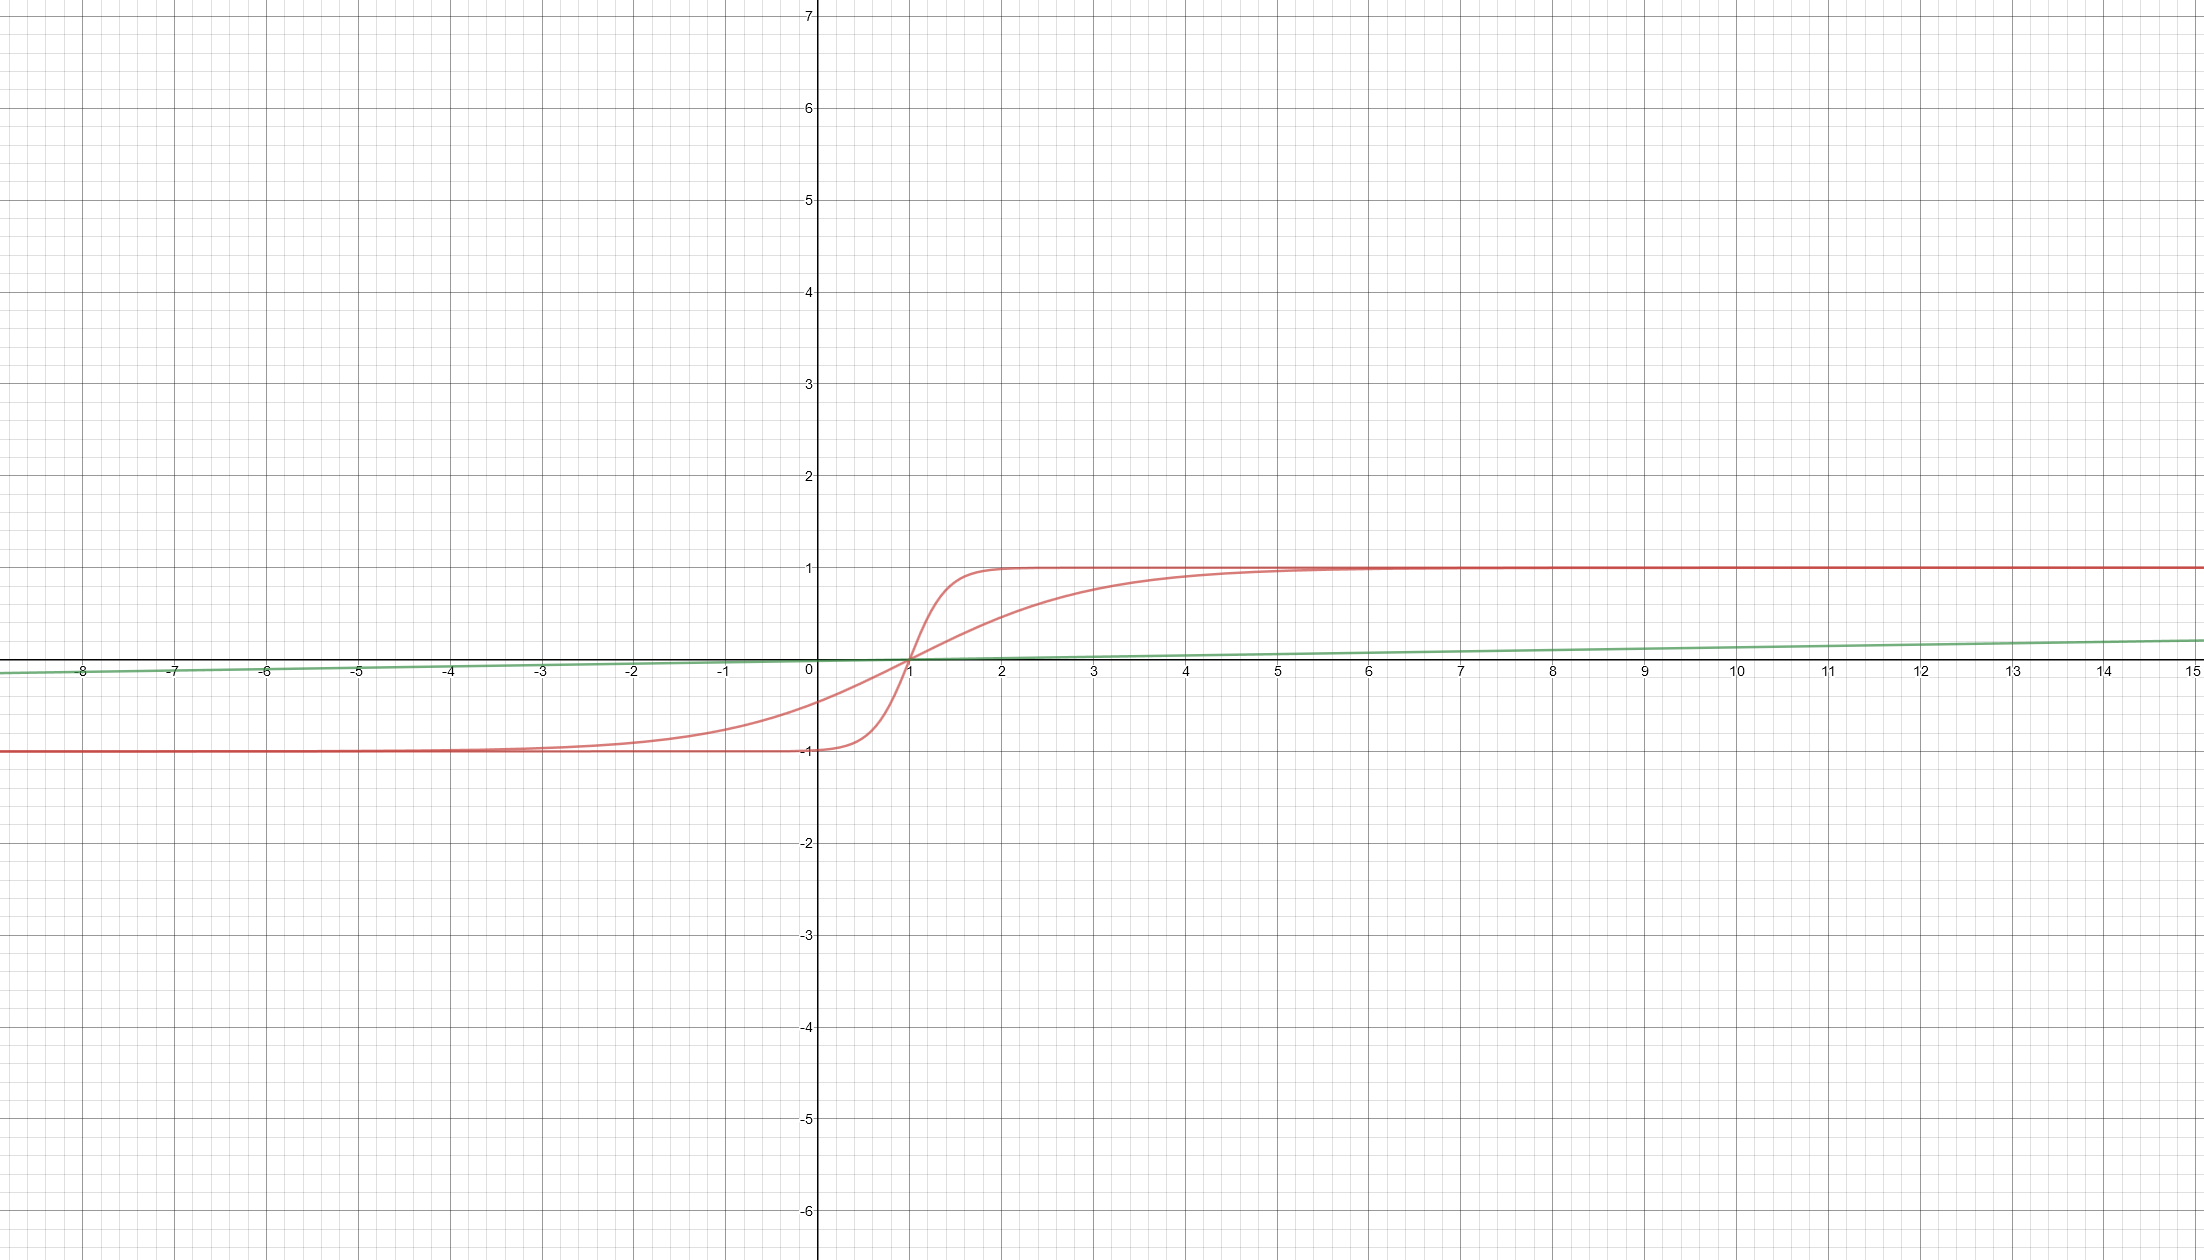
\includegraphics[scale = 0.2]{images/logistic.png}}
	\caption{k = 0.03 in green, k = 1 in bright red, k = 5 in red}
\end{figure}

The normalization process will take place for every dictionary and ratio but they all have to define their own proportional constant.
Every value is stored as a double and the index position of the features a static.




	
	\subsection{Data Sets and Training}
	Beside the labeled repositories in the challenge description we used the additional \hyperref[src:Repositories]{Repositories} provided by a participating team in the official github repository of the InformaticCup 2017 (although you cannot read it: a big thank you at this point!).
	
	\section{Optimizing our Neural Network }

	
	\section{Validation of created Classifier}
	
	\section{Extensions}
	
	
	
	\newpage
	
	\begin{thebibliography}{xxxxxx}
		\bibitem [1] {DukeUniversity} David P. Williams Gaussian Processes (2006) \url{http://people.ee.duke.edu/~lcarin/David1.27.06.pdf}
		\bibitem [2] {ApproximateAnyFunction}  Cybenko., G. (1989) "Approximations by superpositions of sigmoidal functions", Mathematics of Control, Signals, and Systems \url{http://deeplearning.cs.cmu.edu/pdfs/Cybenko.pdf}
	\end{thebibliography}
	
	
	\section{Source Code, used external Libraries and Repositories}
	\paragraph{Source Code}
	Github: \url{https://github.com/Crigges/InformatiCup2017}\\
	\paragraph{Repositories}
	\label{src:Repositories}
	\url{https://github.com/InformatiCup/InformatiCup2017/tree/master/additional_data_sets}
	

\end{document}



